\documentclass[slidestop,compress,mathserif]{beamer}
%\documentclass[slidestop,compress,mathserif,handout]{beamer}

%\documentclass[xcolor=dvipsnames,handout]{beamer}
%\documentclass[xcolor=dvipsnames]{beamer}

%\documentclass[handout]{beamer}

%%% To get rid of solutions on handouts:
\newcommand{\soln}[1]{\textit{\textcolor{darkGray}{#1}}}				% For slides
%\newcommand{\soln}[1]{ }	% For handouts

% to get pausing to work properly on slides
\newcommand{\hide}[1]{#1}	% For slides
%\newcommand{\hide}[1]{ }	% For handouts


%\usepackage{multicol}
\usepackage{amsfonts}
%\usepackage[pdftex,dvipsnames]{color}
\usepackage{graphicx}
\usepackage{subfigure}
%\usepackage{picinpar}
\usepackage{pifont}
\usepackage{pgf,pgfarrows,pgfnodes}
%\usepackage{wasysym,manfnt,phaistos,empheq}
\usepackage[english]{babel}
\usepackage{pgfpages}
\usepackage{natbib}
\usepackage{hyperref}
\usepackage{multimedia}
%\usepackage{amsfonts,amstext,amssymb,amsbsy,amsopn,amsthm,eucal,latexsym,mathrsfs}
\usepackage{amsmath,amsfonts,amstext,amssymb,amsbsy,amsopn,amsthm,eucal,latexsym,mathrsfs}
\usepackage{ulem}
\usepackage{setspace}
\usepackage{array}
%\usepackage{rotating}
\usepackage{multirow}
\usepackage{verbatim}
\usepackage{multicol}

\setbeamertemplate{navigation symbols}{}

%\usepackage{tikz}
%\usetikzlibrary{arrows,shapes,trees,backgrounds}


%\setbeameroption{show notes on second screen}
%\setbeameroption{show notes}
%\setbeameroption{show only notes}

\definecolor{links}{HTML}{2A1B81}
\hypersetup{colorlinks,linkcolor=,urlcolor=links}

\newtheorem*{principle}{Inscrutibility Principle}
\newtheorem*{punchline}{Punch Line}
\newtheorem{defn}{Definition}

\definecolor{Scarlet}{RGB}{140,17,17}
\definecolor{VassarRed}{RGB}{128,0,0}

% "dinglist" environment
  \renewenvironment{dinglist}[2][blue]
  {\begin{list}{\textcolor{blue}{\ding{#2}}}{}}{\end{list}}
  % Symbol definitions for these lists
  \newcommand{\DingListSymbolA}{43}
  \newcommand{\DingListSymbolB}{243}
  \newcommand{\DingListSymbolC}{224}
  \newcommand{\DingListSymbolD}{219}
  \newcommand{\DingListSymbolCheck}{52}
  \newcommand{\DingListSymbolCross}{56}


  \newenvironment{ballotenv}
{\only{%
\setbeamertemplate{itemize item}{\ding{45}}%
\setbeamertemplate{itemize subitem}{\ding{46}}%
\setbeamertemplate{itemize subsubitem}{\ding{46}}}} {}
\setbeamertemplate{itemize item}{\ding{49}}
\setbeamertemplate{itemize subitem}{\ding{47}}
\setbeamertemplate{itemize subsubitem}{\ding{47}}


%User defined colors: See colors section
\xdefinecolor{oiBlue}{rgb}{0.15, 0.35, 0.55}
\xdefinecolor{gray}{rgb}{0.5, 0.5, 0.5}
\xdefinecolor{darkGray}{rgb}{0.3, 0.3, 0.3}
\xdefinecolor{darkerGray}{rgb}{0.2, 0.2, 0.2}
\xdefinecolor{rubineRed}{rgb}{0.89,0,0.30}
\xdefinecolor{linkCol}{rgb}{0.11,0.49,0.95}	
\xdefinecolor{irishGreen}{rgb}{0,0.60,0}	
\xdefinecolor{darkturquoise}{rgb}{0.44, 0.58, 0.86}
\definecolor{lightGreen}{rgb}{0.533,0.765,0.42}
\xdefinecolor{Regalia}{HTML}{522D80}
\xdefinecolor{ClemsonOrange}{HTML}{EA6A20}

\definecolor{duke@LightGrey}{RGB}{200,200,200}\definecolor{DarkGreen}{RGB}{0,100,0}
\definecolor{Oranges}{RGB}{255,127,0}
\definecolor{LightGray}{RGB}{211,211,211}

%\setbeamertemplate{footline}{%
%  \raisebox{5pt}{\makebox[\paperwidth]{\hfill\makebox[10pt]{\scriptsize\insertframenumber}}}}

\setbeamercolor{equation background}{fg=black,bg=duke@LightGrey}
  % Boxed equation
  \newcommand{\eqbox}[2][0.6]{%
  \centerline{
  \begin{beamerboxesrounded}[lower=equation background,width=#1\hsize,shadow=true]{}
\parbox{#1\hsize}{%
      \[
        \textcolor{black} {#2}
      \]}
  \end{beamerboxesrounded}
}}

\AtBeginSection[] {
  \begin{frame}<beamer>\frametitle{Outline}
    \tableofcontents[currentsection,hideothersubsections]
  \end{frame}
}
%
%
%\AtBeginSubsection[] {
%  \begin{frame}<beamer>\frametitle{Outline}
%    \tableofcontents%[currentsection,currentsubsection]
%  \end{frame}
%}

%\usecolortheme[RGB={82,45,128}]{structure}
%\usecolortheme[RGB={162,80,22}]{structure}
\usecolortheme[RGB={128,0,0}]{structure}
\usetheme[secheader]{Boadilla}
%\usetheme[height=7mm]{Rochester}
%\usetheme{Copenhagen}
%\usetheme{Antibes}
%\usecolortheme{seahorse}
%\usecolortheme{crane}
%\usecolortheme{rose}
%\usefonttheme[onlylarge]{structurebold}
%\usefonttheme[onlymath]{serif}



\def\diag{{\rm diag}}


\def\E{\mathbb{E}}
\def\Prob{\mathbb{P}}
\def\argmin{{\rm argmin}}
\def\argmax{{\rm argmax}}
\def\Def{\stackrel{def}{=}}


\newtheorem{assumption}{Assumptions}
\newtheorem*{proposition}{Proposition}
\newtheorem*{remark}{Remark}



%\setbeamercolor{disc title}{bg=oiBlue!40!white!60,fg=blue}
\setbeamercolor{disc body}{bg= Regalia!20!white!80,fg= Regalia!80!black!90}

\setbeamercolor{clicker ungraded title}{bg=irishGreen!80!white!50,fg=irishGreen!30!black!90}
\setbeamercolor{clicker ungraded body}{bg=irishGreen!20!white!80,fg=irishGreen!30!black!90}

\setbeamercolor{clicker review title}{bg=gray!80!white!80,fg=oiBlue!80!black!90}
\setbeamercolor{clicker review body}{bg=gray!30!white!90,fg=oiBlue!80!black!90}

\setbeamercolor{code body}{bg=gray!20!white!80,fg=black}


% Custom commands
\newcommand{\degree}{\ensuremath{^\circ}}
\newcommand{\Note}[1]{
\rule{2.5cm}{0.25pt} \\ \textit{\scriptsize {\textcolor{rubineRed}{Note:} \textcolor{gray}{#1}}}}
\newcommand{\ct}[1]{
\vfill
{\tiny #1}}
\newcommand{\Remember}[1]{\textit{\scriptsize{\textcolor{orange}{Remember:} \textcolor{gray}{#1}}}}
\newcommand{\red}[1]{\textit{\textcolor{rubineRed}{#1}}}
\newcommand{\pink}[1]{\textit{\textcolor{rubineRed!90!white!50}{#1}}}
\newcommand{\green}[1]{\textit{\textcolor{irishGreen}{#1}}}
\newcommand{\webURL}[1]{\urlstyle{same}\textit{\textcolor{linkCol}{\url{#1}}} }
\newcommand{\webLink}[2]{\href{#1}{\textcolor{linkCol}{{#2}}}}
\newcommand{\mail}[1]{\href{mailto:#1}{\textit{\textcolor{linkCol}{#1}}}}
\newcommand{\hl}[1]{\textit{\textcolor{oiBlue}{#1}}}
\newcommand{\hlGr}[1]{\textit{\textcolor{lightGreen}{#1}}}
\newcommand{\mathhl}[1]{\textcolor{oiBlue}{\ensuremath{#1}}}
\newcommand{\ex}[1]{\textcolor{blue}{{{\small (#1)}}}}
\newcommand{\disc}[1]{
\begin{beamerboxesrounded}[shadow = true, lower = disc body, upper = disc title]{}
#1
\end{beamerboxesrounded}
}

\newcommand{\cl}[1]{
\begin{beamerboxesrounded}[shadow = true, lower = clicker ungraded body, upper = clicker ungraded title]{Question}
$\:$ \\
#1
\end{beamerboxesrounded}
}

\newcommand{\clR}[1]{
\begin{beamerboxesrounded}[shadow = true, lower = clicker review body, upper = clicker review title]{\red{Review question} }
$\:$ \\
#1
\end{beamerboxesrounded}
}

\newcommand{\formula}[2]{
\begin{beamerboxesrounded}[shadow = true, lower = white, upper = clicker review body]{#1}
#2
\end{beamerboxesrounded}
$\:$ \\
}

\newenvironment{twocol}[4]{
\begin{columns}[c]
\column{#1\textwidth}
#3
\column{#2\textwidth}
#4
\end{columns}
}


\newenvironment{slot}[2]{
\begin{array}{c}
\underline{#1} \\
#2
\end{array}
}

\newcommand{\pr}[1]{
\left( #1 \right)
}

\newcommand{\solnMult}[1]{
\item[] \vspace{-0.59cm}
\only<beamer| beamer:1>{\item #1}
\soln{\only<2->{\item \red{#1}}}
}

%\newcommand{\codechunk}[1]{
%\begin{beamerboxesrounded}[shadow = true, lower = code body]{}
%{\small #1}
%\end{beamerboxesrounded}
%}

% Change margin

\newenvironment{changemargin}[2]{%
\begin{list}{}{%
\setlength{\topsep}{0pt}%
\setlength{\leftmargin}{#1}%
\setlength{\rightmargin}{#2}%
\setlength{\listparindent}{\parindent}%
\setlength{\itemindent}{\parindent}%
\setlength{\parsep}{\parskip}%
}%
\item[]}{\end{list}}

% Footnote

\long\def\symbolfootnote[#1]#2{\begingroup%
\def\thefootnote{\fnsymbol{footnote}}\footnote[#1]{#2}\endgroup}

% Commands from the book
\newenvironment{data}[1]{\texttt{#1}}{}
\newenvironment{var}[1]{\texttt{#1}}{}
\newenvironment{resp}[1]{\texttt{#1}}{}






%%%%%%%%%%%%%%%%%%%%%%%%%%%%%%%%%%%%%%%%%%%%%%%%%%%%%%%%%%%%%%%%%%%%%%%%%%%%%%%%%%%%%%%%%%%%%%%
\title[Chapter 5 part 1]{Chapter 5 part 1}
\subtitle{Continuous Random Variables}

%%%%%%%%%%%%%%%%%%%%%%%%%%%%%%%%%%%%%%%%%%%%%%%%%%%%%%%%%%%%%%%%%%%%%%%%%%%%%%%%%%%%%%%%%%%%%%%


\author[Jingchen (Monika) Hu] % (optional, use only with lots of authors)
{Jingchen (Monika) Hu}
% - Give the names in the same order as the appear in the paper.
% - Use the \inst{?} command only if the authors have different
%   affiliation.

\institute[Vassar] % (optional, but mostly needed)
{Vassar College}
% - Use the \inst command only if there are several affiliations.
% - Keep it simple, no one is interested in your street address.

\date[MATH 241] % (optional, should be abbreviation of conference name)
{MATH 241}
% - Either use conference name or its abbreviation.
% - Not really informative to the audience, more for people (including
%   yourself) who are reading the slides online

\subject{MATH 241}
% This is only inserted into the PDF information catalog. Can be left
% out.



% If you wish to uncover everything in a step-wise fashion, uncomment
% the following command:

%\beamerdefaultoverlayspecification{<+->}



\begin{document}




%%%%%%%%%%%%%%%%%%%%%

% Title Page

\begin{frame}%[plain]
\titlepage
\end{frame}


%%%%%%%%%%%%%%%%%%%%%%%%%%%%%%%%%%%%%%%%%%
%\addtocounter{framenumber}{-1}
%\begin{frame}{Midterm Feedback}
%\begin{columns}[T]
%\begin{column}{4cm}
%\vspace{-1cm}
%\begin{figure}
%\centering
%\includegraphics[width=5cm,height=8cm]{figures/feedback_barplots}
%\end{figure}
%\end{column}
%\begin{column}{7.8cm}
%\vspace{-0.3cm}
%{\pause
%\small \centerline{\underline{\textbf{Likes}}}}
%{%\footnotesize
%\begin{itemize}
%\item Lecture: well-organized, informative, \\
%clear expectation, good balance between theory and practice
%%in-class questions are  %\\``one of the best math classes"
%\item Slides: well-prepared, easy to follow
%%\item In-class questions: very helpful
%\item Homework \& quizzes: good practice
%\item In-class questions: helpful %in understanding concepts
%\item Exam \& quizzes: fair in difficulty
%\item ``Somewhat challenging but not too much''
%%\item Willingness to help%Available outside of classroom %office hour
%%\item Lab: interesting, practical programming skill, solidify core concepts
%\end{itemize}
%}
%{\pause
%\small \centerline{\underline{\textbf{To improve}}}}
%{%\footnotesize
%\begin{itemize}
%%\item Detailed expectation on the programming software (R) in syllabus
%\item Examples in class: more similar to HW %(harder)
%\item Homework solutions
%\item Practice exam
%%\item Post slides 12 hours before class
%%\item Go over commonly missed homework in class
%%\item Increase participation for in-class questions
%%\item More in-class activities (?)
%%\item More explanation in labs
%%\item More video?
%%\item Slides on Sakai: same slides or handout?
%%\item More practice, more examples
%%\item Some other detailed suggestions...
%
%\end{itemize}
%}
%\end{column}
%\end{columns}
%\end{frame}


%%%%%%%%%%%%%%%%%%%%%%
%\addtocounter{framenumber}{-1}
%
%\begin{frame}\frametitle{Annoucement}
%
%\begin{itemize}
%%\item HW5: \red{due now!}
%\item HW6: \red{due Thursday, Oct 23nd}
%
%\vspace{0.5cm}
%
%
%
%\end{itemize}
%%\begin{center}
%%\includegraphics[width = \textwidth]{figures/midterm_score}
%%\end{center}
%
%
%\end{frame}



%%%%%%%%%%%%%%%%%%%%%%
\begin{frame}{Outline}
%\tableofcontents[hideallsubsections,pausections]
\tableofcontents[hideallsubsections]
\end{frame}


%%%%%%%%%%%%%%%%%%%%%%%%%%%%%%%%%%%%%%%%%%
\section{Continuous random variables}
%%%%%%%%%%%%%%%%%%%%%%%%%%%%%%%%%%%%%%%%%%
\begin{frame}\frametitle{Continuous random variables}

\begin{dinglist}{\DingListSymbolA}
\item A \hl{continuous random variable} $X$ can take any real value in $(-\infty, \infty)$.
\end{dinglist}
\pause
\begin{defn}
$X$ is a continuous random variable if there exists a {\bf nonnegative} function $f$
defined for any $x \in (-\infty, \infty)$, such that for any set $B$ of real numbers,
\[ P(X \in B) = \int_B f(x) dx \]
This function $f$ is called the \hl{probability density function} (pdf) of the random variable $X$.
\end{defn}

\vspace{0.5cm}

\pause
Examples of continuous random variable
\begin{itemize}
\item Rainfall amount for a year.\\
\item Lifetime of your first car. \\
\item Amount of beer consumed on a game day.
\end{itemize}

\end{frame}

%%%%%%%%%%%%%%%%%%%%%%%%%%%%%%%%%%%%%%%%%%
\begin{frame}\frametitle{Pdf and cdf}

\begin{itemize}

\item  For pdf to be valid, in additional to being non-negative,
\[  \int_{-\infty}^{\infty} f(x) dx = P(-\infty < X < \infty) =  1\] \pause

\item Cdf function of continuous random variable
\[ F(a) = P(X \leq a) =  \int_{-\infty}^{a} f(x) dx \]
\pause\vspace{-0.5cm}

\item  For continuous random variable, probability to be a single point is zero.
\[ P(X = a) =   \int_{a}^{a} f(x) dx = 0\]
\[ P(X < a) = P(X \leq a) - P(X = a) = F(a) \]
\pause\vspace{-0.5cm}

\item Probability on an interval
\[ P( a \leq X \leq b) =  F(b) - F(a) = P(a < X < b)\]


\end{itemize}

\end{frame}

%%%%%%%%%%%%%%%%%%%%%%%%%%%%%%%%%%%%%%%%%%
\begin{frame}\frametitle{}
\vspace{-0.5cm}

\begin{center}
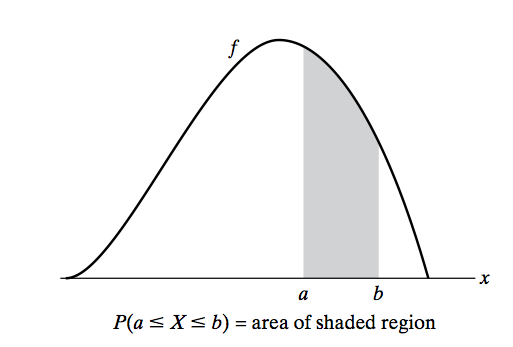
\includegraphics[scale = 0.4]{figures/pdf}
\end{center}
\vspace{-0.3cm}

\pause
Connection between pdf and cdf of continuous random variable. If we know the pdf,
\[ F(a) = P(X \leq a) =  \int_{-\infty}^{a} f(x) dx \]
\pause
How to find the pdf if we know the cdf?


%\invisible{
\vspace{-0.3cm}
\pause
\[ f(x) = \frac{d}{dx}F(x) \]
%}

\end{frame}

%%%%%%%%%%%%%%%%%%%%%%%%%%%%%%%%%%%%%%%%%%
\begin{frame}\frametitle{}
\disc{Example: suppose that $X$ is a continuous random variable whose pdf is
\begin{align*}
f(x) &= \begin{cases}
c (8x - 4 x^3)& \text{if $0 \leq x \leq 1$} \\
0 & \text{otherwise}
\end{cases}
\end{align*}
\vspace{-0.5cm}
\begin{itemize}
\item What's the value of $c$?
%\item Find $P(X > 0.5)$.
%\item Find the cdf function $F(x)$.
\end{itemize}
}

%\invisible{
\pause
\begin{align*}
1  & = \int_{-\infty}^{\infty} f(x) dx\\
& = \int_{0}^{1} c (8x - 4x^3) dx\\
& = c \left( \left. 4x^2 - x^4 \right|_0^1 \right)
\end{align*}
\[ 3c = 1 \Longrightarrow c = \frac{1}{3}  \]
%}


\end{frame}
%%%%%%%%%%%%%%%%%%%%%%%%%%%%%%%%%%%%%%%%%%
\begin{frame}\frametitle{Interpretation of the pdf}
For some small value $h>0$,
\begin{align*}
P\left(x - \frac{h}{2} \leq X \leq x + \frac{h}{2} \right) & = \int_{x - \frac{h}{2}}^{x + \frac{h}{2}} f(t)dt\\
& \approx \left[ (x + \frac{h}{2}) - (x - \frac{h}{2}) \right] f(x)\\
& = h \cdot f(x)
\end{align*}
The larger $f(x)$ is, the more likely $X$ is to be ``near'' $x$.
\end{frame}


%%%%%%%%%%%%%%%%%%%%%%%%%%%%%%%%%%%%%%%%%%
\begin{frame}\frametitle{Recap}

A continuous random variable $X$ can take more than countable number of values in $\mathbb{R}$.
\begin{itemize}
\item We defined continuous random variable using pdf
\[ P(X \in B) = \int_B f(x) dx \]
\pause
\item Cdf function of continuous random variable
\[ F(x) = P(X \leq x) =  \int_{-\infty}^{x} f(t) dt \]
\[ f(x) = \frac{d}{dx}F(x) \]
%\item Expected value of a continuous random variable $X$ with pdf $f(x)$ as
%\[E[X] = \int_{-\infty}^{\infty} x f(x) dx\]
%\[E[g(X)] = \int_{-\infty}^{\infty} g(x) f(x) dx\]
\end{itemize}

\end{frame}

%%%%%%%%%%%%%%%%%%%%%%%%%%%%%%%%%%%%%%%%%%
\section{Expectation and variance of continuous random variable}
%%%%%%%%%%%%%%%%%%%%%%%%%%%%%%%%%%%%%%%%%%
\begin{frame}\frametitle{Expectation and variance of continuous random variable}

\begin{itemize}
\item Recall that expected value of the discrete random variable $X$ with pmf $p(x)$,
\[E[X] = \sum_{\text{all } x} x p(x)\]

\pause
\item We define expected value of a continuous random variable $X$ with pdf $f(x)$ as
\[E[X] = \int_{-\infty}^{\infty} x f(x) dx\]

\pause
\item Definitions of variance and standard deviation are the same.
\[Var(X) = E[X^2] - (E[X])^2, \quad SD(X) = \sqrt{Var{(X)}}  \]
Definition: \[Var(X) = E[(X-\mu)^2] \] 
\end{itemize}

\end{frame}


%%%%%%%%%%%%%%%%%%%%%%%%%%%%%%%%%%%%%%%%%%
\begin{frame}\frametitle{Properties of $E[X]$ for continuous random variable}

\begin{itemize}
\item Recall that expected value of the discrete random variable $X$ with pmf $p(x)$,
\[E[g(X)] = \sum_{\text{all } x} g(x) p(x)\]

\pause
\item Similarly, expected value of a continuous random variable $X$ with pdf $f(x)$ as
\[E[g(X)] = \int_{-\infty}^{\infty} g(x) f(x) dx\]

%\pause
%\disc{Example: show that for non-negative continuous random variable $Y$,
%\vspace{-0.3cm}
%\[ E[Y] = \int_0^{\infty} P(Y>y) dy  \]}
%%\invisible{
%\pause
%%\red{Proof}
%\vspace{-0.3cm}
%\begin{align*}
%\int_0^{\infty} P(Y>y) dy & = \int_0^{\infty} \left[ \int_y^{\infty} f_Y(x)dx \right] dy \\
%& = \int_0^{\infty}   \left[\int_0^{x} dy\right]f_Y(x)dx = \int_0^{\infty} x f_Y(x)  dx = E[Y]
%\end{align*}
%}
%\pause
%{\small{
%\cl{Find $E[e^X]$, if the density function of $X$ is given by
%\begin{align*}
%f(x) &=
%\begin{cases}
%1& \text{if $0 \leq x \leq 1$} \\
%0 & \text{otherwise}
%\end{cases}
%\end{align*}
%}
%
%%\invisble{
%\pause
%$$E[e^X]  = \int_{0}^{1} e^x dx =  e - 1$$
%}}
\end{itemize}


\end{frame}

%%%%%%%%%%%%%%%%%%%%%%%%%%%%%%%%%%%%%%%%%%
\begin{frame}\frametitle{Properties of $E[X]$ for continuous random variable}
Similarly as discrete random variable, for continuous random variable $X$ and $Y$

\begin{itemize}

\item Sum of two random variable's \[ E[X+Y] = E[X]+E[Y] \]


\item If $a$ and $b$ are constants, then
\[ E[aX+b] = a E[X] + b \]

\item If $a$ and $b$ are constants, then
\[ Var(aX+b) = a^2 Var(X) \]

\end{itemize}

\end{frame}

%%%%%%%%%%%%%%%%%%%%%%%%%%%%%%%%%%%%%%%%%%
\begin{frame}\frametitle{}
\disc{Find the mean and variance of the continuous random variable $X$, whose pdf is
\begin{align*}
f(x) &=
\begin{cases}
2x& \text{if $0 \leq x \leq 1$} \\
0 & \text{otherwise}
\end{cases}
\end{align*}
}

%\invisble{
\pause
\begin{align*}
E[X] & = \int_{-\infty}^{\infty} x f(x)dx\\
& =  \int_{0}^{1} x \cdot 2x dx = \left. \frac{2}{3} x^3 \right|_0^1 = \frac{2}{3}
\end{align*}

\pause
\begin{align*}
Var[X] & = E[X^2] - (E[X])^2  = \int_{-\infty}^{\infty} x^2 f(x)dx - (2/3)^2\\
& =  \int_{0}^{1} x^2 \cdot 2x dx - 4/9= \left. \frac{2}{4} x^4 \right|_0^1 - 4/9= \frac{1}{18}
\end{align*}


%}

\end{frame}

%%%%%%%%%%%%%%%%%%%%%%%%%%%%%%%%%%%%%%%%%%
\section{Uniform distribution}
%%%%%%%%%%%%%%%%%%%%%%%%%%%%%%%%%%%%%%%%%%

\begin{frame}
\frametitle{Uniform Distribution}

Let's define a continuous probability distribution that has some constant value $c$ between $\alpha$ and $\beta$
where $\alpha < \beta$. What is the pdf?
\begin{align*}
f(x) &= \begin{cases}
c & \text{if $\alpha < x < \beta$} \\
0 & \text{otherwise}
\end{cases}
\end{align*}


\pause
\[1  = \int_{-\infty}^\infty f(x) dx =\int_{\alpha}^\beta c dx
 = c(\beta - \alpha) \Longrightarrow c = \frac{1}{\beta-\alpha} \]

\pause
\begin{defn}
A continuous random variable $X$ has a \hl{Uniform distribution} on the interval $(\alpha, \beta)$ if its pdf is
\vspace{-0.3cm}
\begin{align*}
X \sim \text{Unif}(\alpha, \beta) \Longleftrightarrow
 f(x) = \frac{1}{\beta-\alpha} \cdot \mathbf{1}_{(\alpha, \beta)}(x) =
\begin{cases}
\frac{1}{\beta-\alpha} & \text{ if } \alpha < x < \beta\\
0 & \text{ otherwise}
\end{cases}
\end{align*}
 \end{defn}

\end{frame}

%%%%%%%%%%%%%%%%%%%%%%%%%%%%%%%%%%%%


\begin{frame}\frametitle{Cdf of Uniform distribution}
For any $x \in (\alpha, \beta)$,
\[
F(x) = \int_{-\infty}^x f(t)~dt
       = \int_{\alpha}^x \frac{1}{\beta-\alpha}~dt
       %= \left. \frac{t}{\beta-\alpha} \right|_a^x
       = \frac{x-\alpha}{\beta-\alpha}
\]

\pause %\vspace{-0.3cm}
\begin{itemize}
\item $X \sim \text{Unif}(\alpha, \beta)$, then its cdf is
%\begin{align*}
$
F(x) =
\begin{cases}
0 & \text{ if } x \leq \alpha\\
\frac{x-\alpha}{\beta-\alpha} & \text{ if } \alpha < x < \beta\\
1 & \text{ if } x \geq \beta
\end{cases}
$
%\end{align*}
\end{itemize}

\pause
\begin{center}
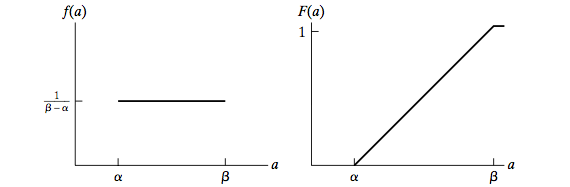
\includegraphics[scale = 0.55]{figures/uniform}
\end{center}



\end{frame}

%%%%%%%%%%%%%%%%%%%%%%%%%%%%%%%%%%%%%%%%%%

\begin{frame}\frametitle{Mean of a Uniform distribution}
\begin{itemize}
\item ({\color{red}required}) Expected value of $X\sim \text{Unif}(\alpha, \beta)$ is
\[ E[X]   = \frac{\alpha + \beta}{2} \]
\end{itemize}
%\red{Proof}

\pause
\begin{align*}
E[X]   &= \int_a^\beta \frac{x}{\beta-\alpha} dx
        = \left. \frac{x^2}{2(\beta-\alpha)} \right|_\alpha^\beta \\
       &= \frac{\beta^2-\alpha^2}{2(\beta-\alpha)} = \frac{\alpha + \beta}{2} \\ \\
\end{align*}




\end{frame}

%%%%%%%%%%%%%%%%%%%%%%%%%%%%%%%%%%%%%%%%%%

\begin{frame}\frametitle{Variance of a Uniform distribution}
\begin{itemize}
\item ({\color{red}required})  Variance of $X\sim \text{Unif}(\alpha, \beta)$ is
\[ Var(X)   = \frac{(\beta - \alpha)^2}{12} \]
\end{itemize}
%\red{Proof}

\pause
\vspace{-0.7cm}
\begin{align*}
E[X^2] &= \int_a^\beta \frac{x^2}{\beta-\alpha} dx
        = \left. \frac{x^3}{3(\beta-\alpha)} \right|_\alpha^\beta \\
       &= \frac{\beta^3-\alpha^3}{3(\beta-\alpha)} = \frac{\beta^2+\beta \alpha+\alpha^2}{3}
\end{align*}
\pause
\begin{align*}
Var(X) &= E[X^2]-E[X]^2 = \frac{\beta^2+\beta \alpha+\alpha^2}{3} - \frac{(\beta+\alpha)^2}{4} \\
       &= \frac{4b^2+4 \beta \alpha+4 \alpha^2}{12} - \frac{3b^2+6 \alpha \beta+3 \alpha^2}{12} \\
       & = \frac{\beta^2-2 \beta \alpha +\alpha^2}{12}
        = \frac{(\beta-\alpha)^2}{12}
\end{align*}



\end{frame}

%%%%%%%%%%%%%%%%%%%%%%%%%%%%%%%%%%%%%%%%%%
\begin{frame}\frametitle{Uniform distribution: probability calculation}

If $X \sim \text{Unif}(\alpha, \beta)$, then
\vspace{-0.8cm}
\[
P(X \in B) = \frac{\text{length}(B)}{\beta - \alpha}
\]

\pause
\disc{Example:  I want to take bus to the airport this afternoon.
The bus arrives at my nearest bus stop at 10-minute intervals starting at 4pm.
Suppose I arrive the bus stop at a time uniformly distributed between 4pm to 5pm.
What's the probability I will wait more than 7 minutes?}

%\invisible{
\pause
Let $X$ denote the time I arrive the bus stop.
\[ X \sim \text{Unif}(0, 60) \]
\pause
The bus arrives at time $t = 0, 10, 20, 30, 40, 50, 60$.\\
So the intervals of my arriving time such that I will wait more than 7 min:
\[
B = (0, 3) \cup (10, 13)  \cup (20, 23) \cup (30, 33) \cup (40, 43) \cup (50, 53)
\]

\pause
\[
P(X \in B)  = (3 \times 6) / 60 = 0.3
\]

%}

\end{frame}


%%%%%%%%%%%%%%%%%%%%%%%%%%%%%%%%%%%%%%%%%%
\begin{frame}\frametitle{Recap}

Expectation for continuous random variable $X$ and a function of it $g(X)$
\[E[X] = \int_{-\infty}^{\infty} x f(x) dx\]
\[E[g(X)] = \int_{-\infty}^{\infty} g(x) f(x) dx\]

\pause

Uniform distribution $X \sim \text{Unif}(\alpha, \beta)$
\twocol{0.5}{0.5}{
\begin{itemize}
\vspace{0.2cm}
\item Pdf \vspace{-0.5cm}
\[f(x) = \begin{cases}
\frac{1}{\beta-\alpha} & \text{ if } \alpha < x < \beta\\
0 & \text{ otherwise}
\end{cases}
 \]
\end{itemize}
}
{
\begin{itemize}
\item Cdf \vspace{-0.6cm}
\[ F(x) =
\begin{cases}
0 & \text{ if } x \leq \alpha\\
\frac{x-\alpha}{\beta-\alpha} & \text{ if } \alpha < x < \beta\\
1 & \text{ if } x \geq \beta
\end{cases}
 \]
\end{itemize}
}
\begin{itemize}
\item Mean and variance  \vspace{-0.2cm}
\[ E[X]   = \frac{\alpha + \beta}{2}, \quad Var(X)   = \frac{(\beta - \alpha)^2}{12} \]
\end{itemize}



\end{frame}




\end{document}
